\documentclass{article}
\usepackage{graphicx,float}
\usepackage{amsmath,latexsym,amsfonts,amssymb,amsthm}

\usepackage[utf8]{inputenc}
\usepackage[english]{babel}
\usepackage[letterpaper,top=2cm,bottom=2cm,left=3cm,right=3cm,marginparwidth=1.75cm]{geometry}
\renewcommand{\baselinestretch}{1.667}


\title{Optimization Without Restrictions - Lab 2}
\author{Joris Plaščinskas}
\date{\today}


\begin{document}


    \maketitle
    \section*{Introduction}
        The goal of this laboratory work was to get familiar with optimization methods without restrictions. In this lab I implemented three methods: gradient descent, steepest descent, deform-able simplex search. The objective was to find the ratio of plots that gives the highest volume. The objective function for this task is negative squared volume: $-V^2 = p_1 \times p_2 \times p_3 \times -1/8$. After making a requirement for the sum of plots to be equal to one, we can derive one plot from the other two, that means that this function is now dependent on two parameters. Since the objective function is very simple and only has one local (and global) minima the results are highly dependent on the parameters. Objective function and its gradient are defined like so in the code:
        \begin{verbatim}
def objective_function(plot_1, plot_2):
    plot_3 = 1 - plot_1 - plot_2
    if (plot_1 < 0 or plot_2 < 0 or plot_3 < 0):
        return float('inf')
    return -(1/8) * plot_1 * plot_2 * plot_3


def objective_gradient_function(plot_1, plot_2):
    return numpy.array([-1/8*(plot_2 - 2*plot_1*plot_2 - plot_2**2), -1/8*(plot_1 - plot_1**2 - 2*plot_1*plot_2)])
        \end{verbatim}
    \section*{Methods and Results}
    Each red dot in the graph's represents a point where the objective function (or it's gradient) was calculated.
        \subsection*{Gradient Descent}
            Gradient descent (learning rate equals 1) converges after 65 iterations with the result: Plot 0: 0.33329781426463617, Plot 1: 0.33329781426463617, Plot 2: 0.3334043714707277, Objective: -0.004629629471940303, Grad: [-5.07344649e-06 -5.07344649e-06]. Which means that it had to calculate the gradient function for 65 times. The code and explanation of gradient descent algorithm is under the figure.
        \begin{figure}[H]
            \centering
            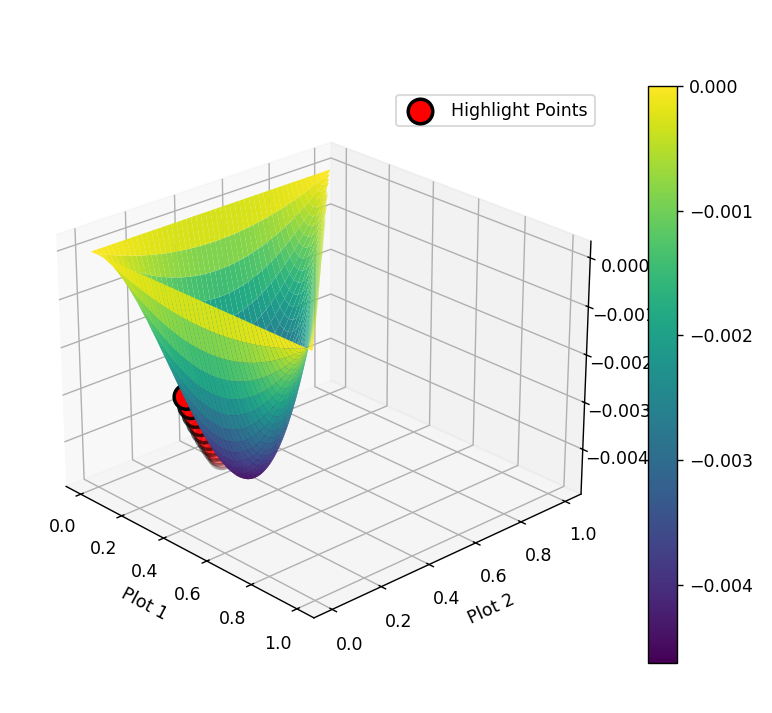
\includegraphics[width=0.5\textwidth]{gradient-02.png}
            \caption{Gradient Descent (0.2, 0.2)}
        \end{figure}
        \begin{verbatim}
def gradient_descent(plot_0, plot_1, step_count=10, learning_rate=1, log=True):
    history = []
    for i in range(step_count):
        history.append((plot_0, plot_1))
        grad = objective_gradient_function(plot_0, plot_1)
        plot_0 -= grad[0] * learning_rate
        plot_1 -=grad[1] * learning_rate

        if log:
            print(f"i = {i} Plot 0: {plot_0}, Plot 1: {plot_1}, Plot 2: {1 - plot_0 - plot_1}, Objective: {objective_function(plot_0, plot_1)}, Grad: {grad}")
            if grad.mean() * learning_rate <= 0.0001:
                print("Small step!")
    
    return history
        \end{verbatim}
        Gradient descent algorithm is an iterative algorithm that takes a step in the direction of the gradient of the objective function. And repeats this until gradient becomes very small or when iterations count is exceeded. Mathematically: $\lim_{k \to \infty} \nabla f(\vec{x}_k) = 0$.

        \subsection*{Steepest Descent}
        Steepest descent converges after 1 (but with 29 iterations during golden ratio search) iteration with the result: Plot 0: 0.3333332600524171, Plot 1: 0.3333332600524171, Plot 2: 0.3333334798951659, Objective: -0.004629629629628959, Grad: [-0.01 -0.01], Step Size: 13.33332600524171. The code implementation and explanation are below the figure.
        \begin{figure}[H]
            \centering
            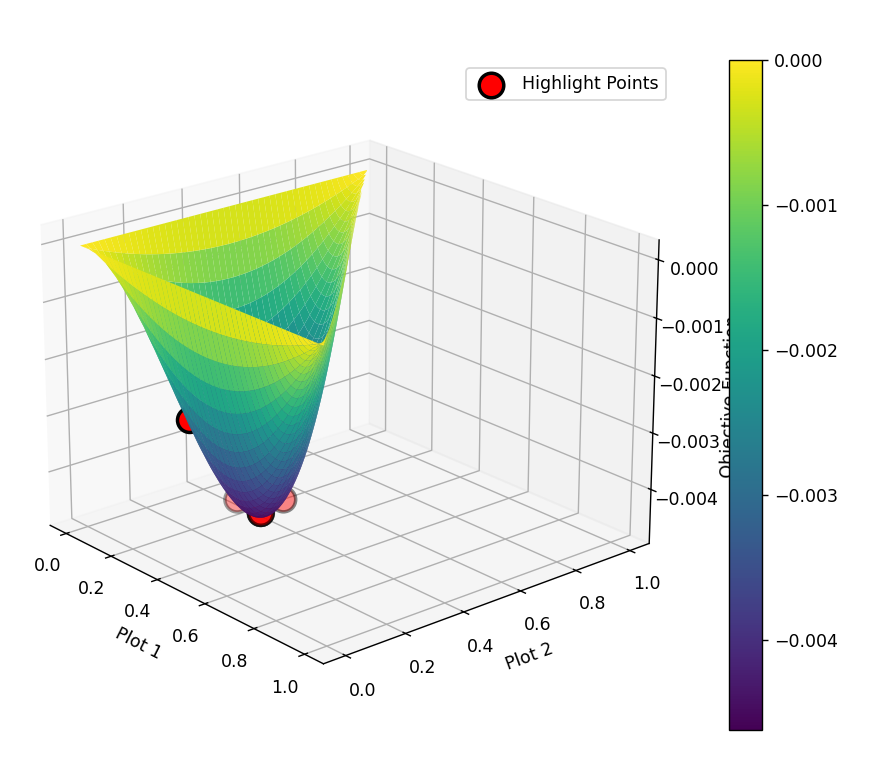
\includegraphics[width=0.5\textwidth]{steepest-02.png}
            \caption{Steepest Descent (0.2, 0.2)}
        \end{figure}
        \begin{verbatim}
def steepest_descent(plot_0, plot_1, step_count=3, log=True):
    history = []
    for i in range(step_count):
        history.append((plot_0, plot_1))
        grad = objective_gradient_function(plot_0, plot_1)

        # Find step size
        one_d_objective = lambda step_size: objective_function(plot_0 - grad[0]*step_size, plot_1 - grad[1]*step_size)
        step_size = one_dimension_optimization.goldenRatioSearchMethod(one_d_objective, 0, 100)
        
        plot_0 -= grad[0] * step_size
        plot_1 -= grad[1] * step_size

        if log:
            print(f"i = {i} Plot 0: {plot_0}, Plot 1: {plot_1}, Plot 2: {1 - plot_0 - plot_1}, Objective: {objective_function(plot_0, plot_1)}, Grad: {grad}, Step Size: {step_size}")
            if grad.mean() * step_size:
                print("Small step!")
        
    return history
        \end{verbatim}
        The idea behind steepest descent is the same as it is for the gradient descent - take a step in the direction of the gradient, and repeat until convergence or step size is exceeded. The difference is that during steepest descent the learning rate (or step size) is dynamically chosen. When the gradient is calculated we can create a new function that takes in only one parameter - the step size and solve 1 dimensional optimization problem, which returns the optimal step size. In this case I used golden ratio search that I implemented during the previous lab.
        \subsection*{Simplex Search}
        Simplex search algorithm converges after 57 iterations with the 3 point coordinates: [(0.33328381587538547, 0.33327097050714244), (0.3332415891470662, 0.33328410951956855), (0.33329901927197314, 0.3333385106720884)]. The code implementation and explanation are below the figure.
        \begin{figure}[H]
            \centering
            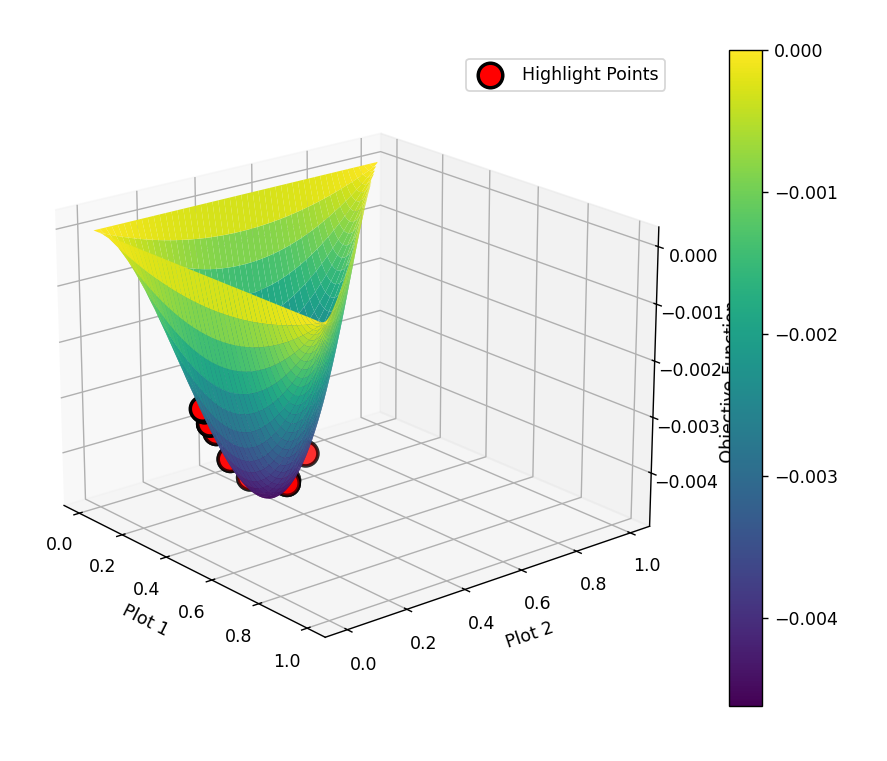
\includegraphics[width=0.5\textwidth]{simplex-02.png}
            \caption{Simplex Search (0.2, 0.2)}
        \end{figure}
        \begin{verbatim}
def simplex_search(point_0=(0.2, 0.2), point_1=(0.21,0.2), point_2=(0.205, 0.21), step_count=10, M=8, scale_factor=2, log=True): # Put the points into an array!
    history = []
    points = [point_0, point_1, point_2]
    point_values = [objective_function(point_0[0], point_0[1]), 
                    objective_function(point_1[0], point_1[1]), 
                    objective_function(point_2[0], point_2[1])]
    reset_counter = [0] * 3

    for i in range(step_count):
        max_index = point_values.index(max(point_values))
        other_indeces = list(range(3))
        other_indeces.remove(max_index)
        highest_p = points[max_index]
        other_p_0 = points[other_indeces[0]]
        other_p_1 = points[other_indeces[1]]
        if any(x > M for x in reset_counter): # Anchoring the highest point (so that I have to write less code..)
            other_p_0 = ((highest_p[0] + other_p_0[0])/2, (highest_p[1] + other_p_0[1])/2)
            other_p_1 = ((highest_p[0] + other_p_1[0])/2, (highest_p[1] + other_p_1[1])/2)

            points[other_indeces[0]] = other_p_0
            points[other_indeces[1]] = other_p_1
            point_values[other_indeces[0]] = objective_function(points[other_indeces[0]][0], points[other_indeces[0]][1])
            point_values[other_indeces[1]] = objective_function(points[other_indeces[1]][0], points[other_indeces[1]][1])

            reset_counter = [0] * 3

            if log:
                print("Shrinked.")
            continue

        center_point = ((other_p_0[0] + other_p_1[0])/2, (other_p_0[1] + other_p_1[1])/2)
        difference = (center_point[0] - highest_p[0], center_point[1] - highest_p[1])

        points[max_index] = (highest_p[0] + difference[0]*2, highest_p[1] + difference[1]*2)
        point_values[max_index] = objective_function(points[max_index][0], points[max_index][1])

        reset_counter[max_index] = 0
        reset_counter[other_indeces[0]] += 1
        reset_counter[other_indeces[1]] += 1

        if point_values[max_index] == min(point_values):
            points[max_index] = (points[max_index][0] + difference[0], points[max_index][1] + difference[1]) # TODO: implement scale factor
            point_values[max_index] = objective_function(points[max_index][0], points[max_index][1])
            if log:
                print("Scaling up.")
        elif point_values[max_index] == max(point_values):
            points[max_index] = (points[max_index][0] - difference[0]*0.5, points[max_index][1] - difference[1]*0.5) # TODO: implement scale factor
            point_values[max_index] = objective_function(points[max_index][0], points[max_index][1])
            if log:
                print("Scaling down.")

        if log:
            print(f"i = {i} Points: {points}, Reset Counter: {reset_counter}")
        
        history.extend(points)
    
    return history
        \end{verbatim}
        Deformable simplex search algorithm is quite different from the previous two. This algorithm doesn't rely on the gradient values instead it works by calculating the objective function. The simplex is initialized with $n+1$ points (when the function has n parameters). Function value is calculated at each point and the worst (highest) point is reflected onto the center of all other points. After reflection if the point is better than the previous best, the simplex expands in that direction. If some point doesn't change more than 8 times the simplex shrinks.
    \section*{Aggregated Results and Conclusion}
        \begin{table}[h!]
            \centering
            \begin{tabular}{|c|c|c|c|}
                \hline
                 & Gradient & Steepest & Simplex \\ \hline
                Calculations & 65 & 30 & 57 \\ \hline
            \end{tabular}
            \caption{Results}
        \end{table}
        The results highly depend on the chosen hyper-parameter values, but Steepest descent showed by far the best performance in this case. The descent algorithms were much easier to implement than simplex. Simplex algorithm might be useful in cases when you don't have access to the gradient function of the objective function.

    
\end{document}